The design of the software, architecture, and technologies used to create the web-application and databases are described in the following section. The analysis being performed by the web-application and how it performs each analysis is discussed and how the back end queries each database.

\subsection{Web-application Simulation}
The web-application, called Providentia\footnote{The name of the web-application is a nod to JanusGraph and Titan's theme of Roman mythology. Providentia is associated with provision and forethought \cite{providentia-meaning}. This was thought to be fitting due to the nature of the experiments bringing out the best database to move forward with when making a decision on which technology to use for storing and modeling one's data.}, is used to queue analysis into a pipeline where each benchmark is to be run, server performance measured, and accumulated results to be displayed. This is deployed on target hardware and will import a subset of the data (given a configurable percentage) and then one will be able to use the web-based interface to perform all necessary benchmarking tasks.

The architecture and how each technology communicates is illustrated in Figure \ref{fig:providentia-architecture}. The databases are containerized using Docker\footnote{\url{https://www.docker.com/}}. 

\begin{figure}[h!]
    \centering
    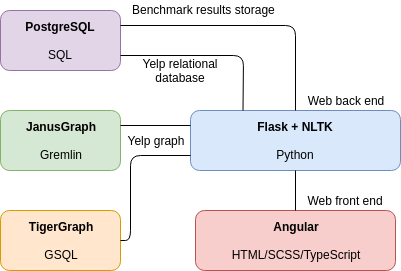
\includegraphics[width=10cm]{img/providentia-architecture.png}
    \caption{The architecture of Providentia.}
    \label{fig:providentia-architecture}
\end{figure}

JanusGraph has some Java specific features that add limitations when making use of embedded Gremlin in Python. These limitations are when trying to make use of mixed indexing search predicates such as spatial queries. The workaround for this was making use of the Gremlin Translator which would take Gremlin as a string and interpret it on the server side.

The first motivation towards using a Python back end is that the text in the reviews can be analysed using NLTK for easy sentiment analysis. The second is that a simple REST API can easily and quickly be designed using the Flask framework. Angular was subjectively chosen as the front end framework as it allows for fast and stable front end web development. All benchmark results are stored in a separate database within PostgreSQL.

The front end of Providentia allows a user to query each database, test the sentiment classifier, add benchmarking jobs and to review the performance and results of each analysis. Each job is run serially to avoid too much interference and competition between each database for resources. At intervals the CPU performance and memory consumption is measured and stored in PostgreSQL. The server performance and results of an analysis can be viewed together to validate that the outputs are the same and how each database uses the server's resources.

\subsection{Data Analysis}
Over each of the databases a number of data analysis jobs are performed on the data. This section describes what each analysis aims to do and how they align to a typical real world use case. Each of these jobs have some kind of spatiotemporal aspect to test the accessibility of the data to demonstrate how well the given database handles the data. 

These analysis are run over different percentages of the data loaded in each database and the performance is then measured and discussed in Section \ref{sec:experiments}. This section goes into more detail about the types of queries written and how well each language expresses each query.

\subsubsection{Kate's Restaurant Recommendation Analysis}
\textcolor{blue}{ TODO: Discuss analysis simulation and language processing involved.}

\subsubsection{Review Trends in Phoenix 2018 Analysis}
\textcolor{blue}{ TODO: Discuss analysis simulation and language processing involved.}

\subsubsection{\textcolor{blue}{ TODO: Come up with a third analysis.}}
\textcolor{blue}{ TODO: Discuss analysis simulation and language processing involved.}

\subsection{Database Technologies}

This section covers the underlying technologies used to implement the databases being benchmarked. This is important to note in terms of how portable each technology is, how difficult the configuration is before each database can be used for a given project, or limitations on performance or hardware requirements due to software requirements.

\subsubsection{PostgreSQL}
PostgreSQL is written in the C programming language and is an object-oriented relational database.
\textcolor{blue}{ TODO: Discuss PostgreSQL.}
\subsubsection{JanusGraph}
\textcolor{blue}{ TODO: Discuss JanusGraph.}
\subsubsection{TigerGraph}
\textcolor{blue}{ TODO: Discuss TigerGraph.}